\documentclass[11pt, a4paper]{article}
\usepackage{natbib}
\usepackage{eso-pic}
\usepackage{amsmath} % flere matematikkommandoer
\usepackage{amssymb}
\usepackage[utf8]{inputenc} % æøå
\usepackage[T1]{fontenc} % mere æøå
\usepackage[danish, english]{babel} % orddeling
\usepackage{verbatim} % så man kan skrive ren tekst
\usepackage{listings}
\usepackage{graphicx}
\usepackage{booktabs}
\usepackage{enumitem}
\usepackage{placeins}
\usepackage[colorlinks=false]{hyperref}
\usepackage{tocbibind}
\usepackage{fancyvrb}

% Default fixed font does not support bold face
\DeclareFixedFont{\ttb}{T1}{txtt}{bx}{n}{10} % for bold
\DeclareFixedFont{\ttm}{T1}{txtt}{m}{n}{10}  % for normal

% Custom colors
\usepackage{color}
\definecolor{deepblue}{rgb}{0,0,0.5}
\definecolor{deepred}{rgb}{0.6,0,0}
\definecolor{deepgreen}{rgb}{0,0.5,0}

% Python style for highlighting
\newcommand\pythonstyle{\lstset{
        language=Python,
        basicstyle=\ttm,
        otherkeywords={self},             % Add keywords here
        keywordstyle=\ttb\color{deepblue},
        emph={MyClass,__init__},          % Custom highlighting
        emphstyle=\ttb\color{deepred},    % Custom highlighting style
        stringstyle=\color{deepgreen},
        frame=tb,                         % Any extra options here
        showstringspaces=false            %
    }}


% Python environment
\lstnewenvironment{python}[1][]
{
    \pythonstyle
    \lstset{#1}
}
{}

% Python for external files
\newcommand\pythonexternal[2][]{{
        \pythonstyle
        \lstinputlisting[#1]{#2}}}

% Python for inline
\newcommand\pythoninline[1]{{\pythonstyle\lstinline!#1!}}

\author{
    Christian Kjær Larsen \texttt{(011292)} \\[.4cm]
    Lukas Svarre Engedal \texttt{(210790)} \\[.4cm]
    Tobias Sønderskov Hansen \texttt{(240395)} \\[.4cm]
    Instruktor: Aske Mottelson\\[.4cm]
    \vspace{9cm}
}

\title{
  \vspace{3cm}
  \Huge{Projektkursus i Systemudvikling 2015} \\[.10cm]
  \Large{PoP-Webhelp}
}

\date{}

\begin{document}
\selectlanguage{danish}
\AddToShipoutPicture*{\put(0,0){\includegraphics*[viewport=0 0 700 600]{includes/nat-farve}}}
\AddToShipoutPicture*{\put(0,602){\includegraphics*[viewport=0 600 700 1600]{includes/nat-farve}}}

%% Change `ku-en` to `nat-en` to use the `Faculty of Science` header
\AddToShipoutPicture*{\put(0,0){\includegraphics*{includes/nat-en}}}

\clearpage\maketitle
\thispagestyle{empty}

\newpage

\selectlanguage{english}
\begin{abstract}
This report presents the development of an e-learning system for use in the newly created introductory computer science course at the Department of Computer Science at University of Copenhagen, called \emph{Programmering og Problemløsning}(Programming and Problemsolving). Our clients are Martin Dybdal and Oleksandr Shturmov, both employed at the department, who will be responsible for the course. In the course, the students will be taught the programming language \verb!F#!.

The aim of the e-learning system is to introduce new students to programming in a simple and user-friendly way, and to teach them various basic ideas and concepts in programming in general, and \verb!F#! in particular. This is done by presenting the students with a series of different exercises, sorted based on subject and difficulty, and presented to students in a specific and meaningful order.

The system will have two different kinds of users; students and admins.
Students will mainly be working on the various exercises, and they will also be able to get hints for the exercises if needed and provide feedback on the exercises and hints once completed. Students should also be able to see how well they are doing so far, for instance how many of the exercises belonging to a particular subject matter they have solved.

The primary role of the admins will be managing the exercises and supervising how well the students are doing. They should be able to easily delete or modify existing exercises or add new ones, as well as manage the order in which the students are presented with the exercises. They should also be able to get various statistics about how the students are doing in order to improve and optimize the exercises, their order and their subjects.
\end{abstract}
\selectlanguage{danish}

\newpage
\section*{Indholdsfortegnelse}
\label{sec:toc}
\makeatletter
\@starttoc{toc}
\makeatother

\thispagestyle{empty}

\newpage
\pagestyle{plain}
\setcounter{page}{1}
\pagenumbering{arabic}

\section{Review}

\subsection{Programming as theory building}
\label{sub:programming_as_theory_building}

\subsection{Extreme Programming}
\label{sub:extreme_programming}

\newpage

\section{Formål og rammer}
\label{sec:formal_og_rammer}
I dette afsnit beskrives systemets formål og rammer ved \textit{FACTOR}-kriteriet, !!!citat mangler!!!, samt centralt terminologi forklares.

\subsection{FACTOR}
\label{sub:factor}
\paragraph{Funktionalitet}
\begin{itemize}
    \item Besvare programmeringsspørgsmål
    \item Oprette programmeringsspørgsmpl
    \item Analysere de studerendes fremskridt
    \item Håndtere de studerendes login
\end{itemize}
\paragraph{Anvendelsesområde}
\begin{itemize}
    \item Undervisere ved DIKU
    \item Førsteårsstuderende ved DIKU
\end{itemize}
\paragraph{Betingelser}
\begin{itemize}
    \item Undervisere har begrænsede resurser
    \item Det skal foregå online
\end{itemize}
\paragraph{Teknologi}
\begin{itemize}
    \item Python 2.7
    \item Flask webframework
    \item SQLAlchemy
    \item HTML/CSS
    \item JavaScript
\end{itemize}
\paragraph{Objekter}
Studerende, Spørgsmål, Hint, Underviser.
\paragraph{Ansvar}
E-læringssystem der skal hjælpe de studerende med programmering.

\subsection{Terminologi}
\label{sub:terminologi}


\section{Kravspecifikation}
\label{sec:kravspecifikation}
I dette afsnit beskrives kravene til systemet, delt op i de funktionelle og de ikke-funktionelle krav. Der er også diagrammer der uddybber systemets funktionalitet og udformning.

\subsection{Krav}
\label{sub:krav}
\paragraph{Funktionelle krav}
De funktionelle krav for systemet er i tråd med afsnit 4.3.1 i \cite{OOSE}, nemlig at de omhandler den specifikke brug af systemet.
\begin{itemize}
    \item Systemet skal være en hjemmeside med opgaver, som kan løses individuelt af de studerende.
    \item Der kræves login, så man kan følge med i den studerendes udvikling.
    \item Spørgsmålene skal være grupperede efter hvilke læringsmål de tester.
    \item Læringsmålene skal igen grupperes i nogle blokke, hvor idéen så er at man gennemgår blokkene én af gangen i en bestemt rækkefølge, og at sværhedsgraden stiger løbende.
    \item Der skal være hints til opgaverne som de studerende kan benytte om nødvendigt, og de studerende skal kunne give feedback til disse hints.
    \item Alle forsøg på opgavebesvarelser skal gemmes i en log.
\end{itemize}

Hvis der er tid i en af de senere iterationer, så er der en del ekstra funktionalitet som kan implementeres.
\begin{itemize}
    \item Loggen skal bruges til at give underviseren information om hvilke spørgsmål der er svære.
    \item Der skal tilføjes en grad af \emph{gamification}, så der gives badges og point for fremskridt, og det bliver muligt at følge med i andres fremskridt.
    \item Hvis man ikke har øvet sig i et emne i et stykke tid, så falder ens erfaring i området.
\end{itemize}

\paragraph{Ikke-funktionelle krav}
\label{par:ikke_funktionelle_krav}
I afsnit 4.3.2 i \cite{OOSE} beskrives ikke-funktionelle krav som krav, der ikke direkte beskriver funktionaliteten, men som er mere generelle krav omkring aspekter som brugervenlighed, ydeevne, pålidelighed og hvor vedligeholdesesvenligt systemet er.

De ikke-funktionelle krav til dette projekt er forholdsvis begrænsede, idet vi har fået forholdsvis stor frihed i forhold til hvordan vi løser opgaven af vores kunde.

\begin{itemize}
\item Det skal være simpelt og hurtigt at tilføje nye opgaver til systemet, sådan at kursuslederne efterfølgende kan opbygge en tilstrækkelig samling af opgaver til de studerende.
\item Det endelige produkt skal gerne skal være simpelt og modulært, sådan at det er nemt at overtage, udvide og bygge videre på efter at vi overgiver projektet til kunden.
\item Ingen af kunderne er web-udviklere, så det er også vigtigt at det valgte framework er veldokumenteret, samt at det er til at gå i gang med at bruge uden at skulle sætte sig ind i store mængder funktionalitet og dokumentation.
\end{itemize}

\subsection{Use case model}
\label{sub:use_case_model}
På Figur \ref{fig:use_case_model} kan man se vores use case model diagram. Vi har at gøre med to aktører, nemlig studerende og administratorer. Det vigtige for studerende er at de kan oprette sig på siden, og at de har adgang til opgaver de kan besvare. Det vigtige for administratorer er at de kan administrere opgaverne, og at de kan få feedback og statistik på hvordan de studerende klarer opgaverne. Begge aktører skal desuden kunne benytte simpel funktionalitet i forbindelse med deres login.

\begin{figure}[h]
  \centering
  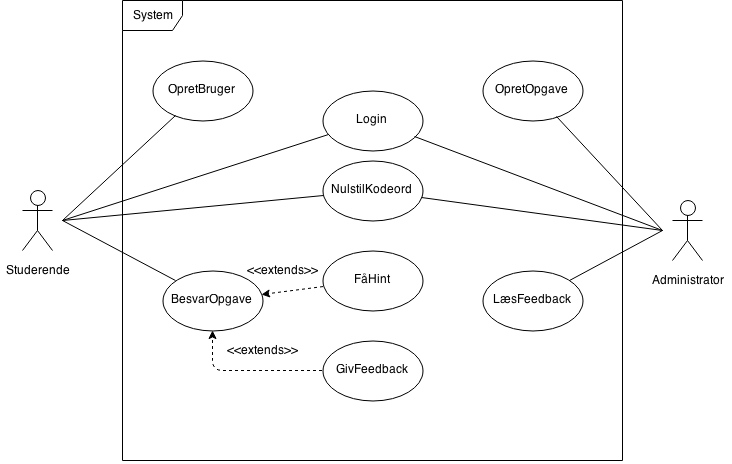
\includegraphics[width=1\linewidth]{figures/UseCaseModel.png}
  \caption{Use case model for vores system.}
  \label{fig:use_case_model}
\end{figure}
\FloatBarrier

\subsection{Use cases}
\label{sub:use_cases}
På Figur \ref{fig:use_case1} ses en beskrivelse af use casen, hvor en studerende opretter sin bruger. Det er en simpel use case, der beskriver i detaljer hvordan processen med at oprette sig som bruger i systemet skal foregå. Inden denne use case er brugeren ikke oprettet i systemet, og når use casen er fuldført har brugeren oprettet sig, er godkendt og er logget ind. Det kombinerer en del af funktionaliteten i én use case. Det kunne godt deles op, men da vi her kun skal beskrive tre overordnede use cases, så har vi valgt at kombineret dem.

\begin{figure}[h]
    \centering
    \begin{tabular}{r p{8cm}}
        \toprule
        \textit{Navn på use-case:} & \verb!OpretBruger! \\
        \hline
        \textit{Deltagende aktører:} & Påbegyndt af en studerende \\
        \hline
        \textit{Hændelser:} & \begin{enumerate}[nolistsep]
            \item En studerende åbner hjemmesiden og klikker på \verb!register!
            \item Den studerende indtaster sine brugeroplysninger, dvs. ku-id og kodeord.
            \item Systemet opretter brugeren, og sender en e-mail med et aktiveringslink.
            \item Den studerende går ind på sin ku-mail klient, åbner mailen og klikker på linket, hvilket aktiverer kontoen.
            \item Den studerende bringes til login-siden.
            \item Den studerende indtaster ku-id og kodeord og klikker \verb!Login!
            \item Der informeres om succesfuldt login, og brugeren bringes til forsiden.
        \end{enumerate}  \\
        \hline
        \textit{Startbetingelse:} & Den studerende har ingen konto, og er ikke logget ind. \\
        \hline
        \textit{Slutbetingelse:} & Den studerende har en aktiveret konto og er logget ind. \\
        \bottomrule
    \end{tabular}
    \caption{Use case omkring oprettelse af bruger.}
    \label{fig:use_case1}
\end{figure}

På Figur \ref{fig:use_case2} ses en beskrivelse af use casen, hvor en studerende svarer på spørgsmål inden for et givet subject. Når den studerende har valgt et subject vil vedkommende blive stillet en række af spørgsmål tilhørende dette subject. Hver gang den studerende svarer rigtigt på et spørgsmål bliver vedkommende belønnet med point. Dette fortsætter indtil har opnået nok point til at gennemføre det givne subject. 

\begin{figure}[h]
    \centering
    \begin{tabular}{r p{8cm}}
        \toprule
        \textit{Navn på use-case:} & \verb!BesvarSpørgsmål! \\
        \hline
        \textit{Deltagende aktører:} & Påbegyndt af en studerende \\
        \hline
        \textit{Hændelser:} & \begin{enumerate}[nolistsep]
            \item Den studerende åbner hjemmesiden.
            \item Vedkommende vælger et subject inden for et threshold der er låst op ved at have færdiggjort det forrige.
            \item Systemet præsenterer et spørgsmål for den studerende. Der kan være flere typer spørgsmål (multiple-choice, udfyldning med flere).
            \item Den studerende angiver sit svar.
            \item Systemet giver respons på svaret, og gemmer det i loggen.
            \item Den studerende trykker næste, for at få et spørgsmål mere.
            \item Når den studerende har svaret på nok spørgsmål, har vedkommende gennemført det aktuelle subject, og tages tilbage til forsiden.
        \end{enumerate}  \\
        \hline
        \textit{Startbetingelse:} & Den studerende er logget ind. \\
        \hline
        \textit{Slutbetingelse:} & Den studerende har gennemført et subject. \\
        \bottomrule
    \end{tabular}
    \caption{Use case omkring besvarelse af spørgsmål og gennemførelse af subject.}
    \label{fig:use_case2}
\end{figure}

Et af kravene for systemet er, at det skal være enkelt og hurtigt for underviserne i kurset at oprette nye spørgsmål. Da underviserne selv er dataloger, så vil det være optimalt hvis man kan lave spørgsmålene i et struktureret filformat. Vi er blevet enige om at bruge \verb!YAML!\footnote{\url{http://yaml.org}}, derfor er use-casen på Figur \ref{fig:use_case3} meget simpel, og består kun af upload af en YAML fil. Filen der uploades bliver i virkeligheden ikke gemt nogen steder, den bliver bare læst og dataene bliver så brugt til at oprette det nye spørgsmål.

\begin{figure}[h]
    \centering
    \begin{tabular}{r p{8cm}}
        \toprule
        \textit{Navn på use-case:} & \verb!OpretOpgave! \\
        \hline
        \textit{Deltagende aktører:} & Påbegyndt af en administrator \\
        \hline
        \textit{Hændelser:} & \begin{enumerate}[nolistsep]
            \item Administratoren trykker på \verb!Upload File!.
            \item En YAML fil uploades i en formular.
            \item Serveren læser filen og opretter spørgsmålet.
            \item Administratoren informeres om at spørgsmålet er oprettet.
        \end{enumerate}  \\
        \hline
        \textit{Startbetingelse:} & En administrator der er logget ind. \\
        \hline
        \textit{Slutbetingelse:} & Det nye spørgsmålet er oprettet. \\
        \bottomrule
    \end{tabular}
    \caption{Use case omkring oprettelse af opgaver.}
    \label{fig:use_case3}
\end{figure}
\FloatBarrier

\subsection{Klassediagram}
På Figur \ref{fig:class_diagram} kan man se vores klassediagram. Størstedelen af klasserne har at gøre med opgaverne og deres inddeling i forskellige grupper samt de forskellige typer af opgaver der findes. Derudover er der et par klasser der har at gøre med den log der føres over de studerendes opgavebesvarelser, for at de kursusansvarlige kan følge med i hvad der går godt og mindre godt. Endeligt er der en klasse for brugere af systemet.

\begin{figure}[h]
    \centering
    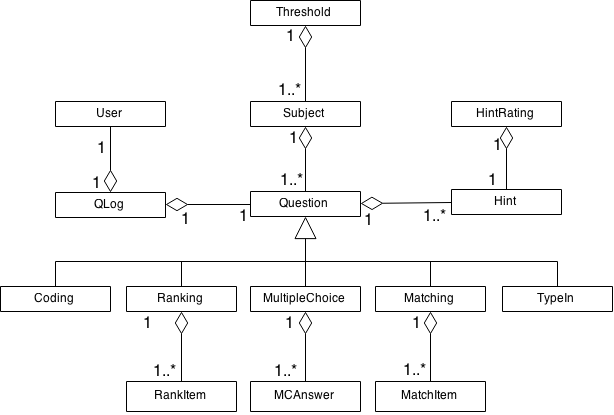
\includegraphics[width=0.8\linewidth]{figures/ClassDiagram.png}
    \caption{Klassediagram af problemområdet}
    \label{fig:class_diagram}
\end{figure}
\FloatBarrier

\subsection{BCE-model}
På Figur \ref{fig:bce_model} kan man se vores BCE model. Modellen har to entity-objekter, fire controller-objekter samt tre boundary-objekter.

\begin{figure}[h]
  \centering
  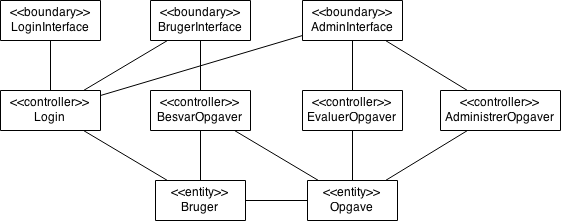
\includegraphics[width=0.8\linewidth]{figures/BCE-Model.png}
  \caption{BCE model for vores system.}
  \label{fig:bce_model}
\end{figure}

De to entity-objekter er \emph{Bruger} og \emph{Opgave}. \emph{Bruger} indeholder informationer om hver enkelt bruger, så som login-oplysninger, hvor vidt brugeren er studerende eller admin samt hvilke opgaver brugeren allerede har løst. \emph{Opgave} indeholder alle informationerne om de enkelte opgaver, det er både selve opgaven der skal løses samt statistik omkring hvordan det er gået når studerende har løst opgaven.

Modellen har tre boundary-objekter, hvor det første man vil møde når man indlæser siden er \textit{login}-brugergrænsefladen, der sammen med \emph{login}-controlleren sørger for at logge brugerne ind i systemet. Derefter vil man så enten have adgang til \emph{Bruger}-grænsefladen eller \emph{Admin}-grænsefladen afhængig af hvad ens status er, og derfra har man adgang til en række controllers.

Modellen har fire controller-objekter, hvor den første er \emph{login}-controlleren der som tidligere nævnt står for at logge brugere ind i systemet. Som studerende vil man have adgang til \emph{BesvarOpgave}-controlleren, der snakker sammen med \emph{Bruger} og \emph{Opgave} og sørger for at stille brugeren de rigtige opgaver. Som admin vil man have adgang til to controllers, nemlig \emph{EvaluerOpgave}-controlleren og \emph{AdministrerOpgave}-controlleren. \emph{EvaluerOpgave}-controlleren snakker sammen med \emph{Opgave} og giver en adgang til de forskellige slags statistik der bliver samlet om opgaverne, og \emph{AdministrerOpgave}-controlleren snakker ligeledes sammen med \emph{Opgave} og giver en adgang til at slette eller ændre i eksisterende opgaver samt tilføje nye.
\FloatBarrier

\subsection{Sekvens-diagrammer}
I dette afnit er der lavet sekvensdiagrammer over de tre use cases der er beskrevet i Afsnit \ref{sub:use_cases}. De funktionskald der fremgår af sekvensdiagrammerne er ikke nødvendigvis reelle funktioner i vores applikation, men er nærmere brugt for at beskrive hvad der sker.
På Figur \ref{fig:opret_bruger_sekvens} kan man se sekvens-diagrammet for den første use case, der beskriver hvordan en studerende opretter sig som bruger i systemet. Her indgår to adskilte sessioner. I den første opretter brugeren sig i systemet, og systemet så sender en email til brugeren. I næste session klikker brugeren på et link i denne email, og brugeren bliver så aktiveret i systemet. Derefter logger brugeren ind, får at vide at det er lykkedes, og use casen er så færdig.

\begin{figure}[h]
    \centering
    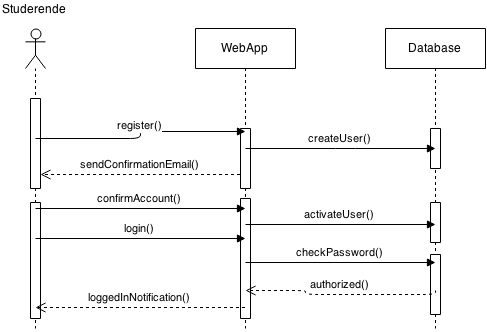
\includegraphics[width=0.8\linewidth]{figures/OpretBrugerUseCase.png}
    \caption{Sekvensdiagram over opretning af bruger}
    \label{fig:opret_bruger_sekvens}
\end{figure}

På Figur \ref{fig:svar_sekvens} kan man se sekvens-diagrammet for den anden use case, der beskriver hvordan en studerende vælger et subject og dernæst besvarer spørgsmål indtil subject'et er gennemført. Løkken viser at der kan komme flere end ét spørgsmål efter det første.

\begin{figure}[h]
    \centering
    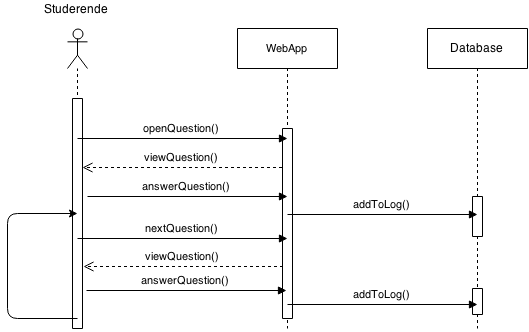
\includegraphics[width=0.8\linewidth]{figures/SvarUseCase.png}
    \caption{Sekvensdiagram over besvarelse af spørgsmål og gennemførelse af subject.}
    \label{fig:svar_sekvens}
\end{figure}

På Figur \ref{fig:opret_sp_sekvens} kan man se sekvens-diagrammet for den tredje use case, der beskriver hvordan en administrator opretter et nyt spørgsmål i systemet. Dette sekvensdiagram er stort set linært, da der ikke sker mere end at der uploades fil, filen læses og spørgsmålet tilføjes, og der gives respons om hvorvidt at spørgsmålet er oprettet korrekt.

\begin{figure}[h]
    \centering
    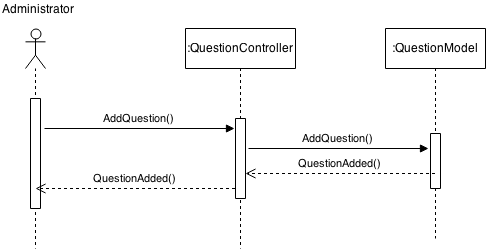
\includegraphics[width=0.8\linewidth]{figures/OpretSporgsmalUseCase.png}
    \caption{Sekvensdiagram over opretning af spørgsmål}
    \label{fig:opret_sp_sekvens}
\end{figure}
\FloatBarrier

\section{Systemdesign}
\label{sec:systemdesign}

I dette afsnit beskrives de designopgaver der er udført allerede. Til sidst i afsnittet gennemgås de dele der endnu ikke er udført.

\subsection{Valg af frameworks}
\label{sub:valg_af_frameworks}

Som før omtalt i Afsnit~\ref{sec:formal_og_rammer} har vi valgt at bruge frameworket Flask som grundlag for vores webapplikation, der på deres egen hjemmeside\footnote{\url{http://flask.pocoo.org/}} er beskrevet som et såkaldt \emph{microframework}. Det betyder at der ikke følger mange af de ting med som der gør i mange større webframeworks. Flask tilbyder kun HTTP routing og templating. Resten skal man selv finde andre biblioteker til. Vi har valgt det, da der så ikke er så meget, at skulle sætte sig ind i, og det giver mere frihed til at udforme applikationen som kunden og vi synes er bedst.

\subsection{Strukturering}
\label{sub:strukturering}

I nogle udviklingsmiljøer er der typisk givet en struktur af kodebasen på forhånd. Det gælder f.eks. mange gange når man bruger store frameworks som Django til Python eller Play til Java. Der er nogle konventioner til hvilke klasser der skal i hvilke mapper, og til hvordan konfigurationsfiler skal struktureres. Det er med til at sikre en god strukturing af koden. Frameworket Flask, som vi har valgt at bruge, har ikke sådanne konventioner. Alt kode kunne placeres i en stor fil hvis man ville. Derfor har vi været omhyggelige med at organisere moduler og klasser på en sådan måde at det er nemt at finde hoved og hale i.

Det giver god mening som den første nedbrydning at dele applikationen op i moduler, som hver især indkapsler adskildt funktionalitet. Det beskrives også i kapitel 6.3 i \cite{OOSE}, hvor det beskrives hvordan man får delt et system op, så kohæsionen mellem moduler bliver så lille som mulig. Ud fra kravspecifikationen har vi nedbrudt det i fire moduler; \texttt{user, admin, question} og \texttt{log}. 

\texttt{User} modulet håndterer den del der har at gøre med brugerlogins, og alt der hører med af oprettelse, ændring af kodeord, nulstilning af kodeord osv. \texttt{Admin} modulet håndterer den del der har at gøre med administration af spørgsmål, subects, thresholds og brugere. \texttt{Log} modulet håndterer den del der har at gøre med logning af statistik fra spørgsmålbesvarelser, samt visning af denne. Endlig håndterer \texttt{question} modulet den del der har at gøre med spørgsmål, både selve opbygningen af hele spørgsmål-strukturen samt visning og besvarelse af spørgsmål.

Det har gjort at vi har kunnet takle problemer uafhængigt af hinanden, og derved har kunnet udvikle mere effektivt.

\subsection{Databasedesign}
\label{sub:databasedesign}
På Figur \ref{fig:er_diagram_question} er ER-diagrammet for hele spørgsmål-aspektet af vores database. Det er minder en del om klassediagrammet over vores problemområde som ses på Figur \ref{fig:class_diagram}, dog er det her mere konkret vist hvilke atributter de enkelt klasser har. På diagrammet ses strukturen for hvordan spørgsmålene er inddelt. Man kan se hvordan et \emph{Question} hører til et \emph{Subject}, der igen hører til et \emph{Threshold} og så videre. Vi prøver også at vise den modulære struktur hvor vi har ladet nye typer spørgsmål nedarve fra den generaliserede type.

\begin{figure}[h]
    \centering
    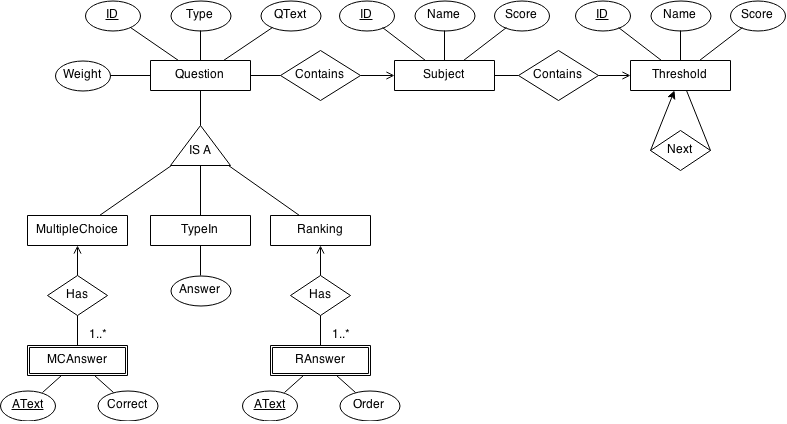
\includegraphics[width=0.8\linewidth]{figures/er_diagram/Qdb.png}
    \caption{ER-diagram over delen af databasen hvor spørgsmålene hører til.}
    \label{fig:er_diagram_question}
\end{figure}

Log-aspektet af vores database er rimelig simpel, idet at vi helt simpelt har to tabeller; QLog og HintRatings. Hver gang en studerende vælger et emne og begynder at svare på spørgsmål bliver der gemt en masse informationer om det i QLog-tabellen. I den anden tabel bliver det gemt når en studerende giver en vurdering af et specifikt hint.

Det tredje aspektet af vores database er brugere. Vi har en User tabel, hvor alt informationen om de studerende og deres kontoer bliver gemt, samt informationer om admins.
\FloatBarrier

\subsection{Brugere}
\label{sub:brugere}

Modulet \texttt{user} håndterer brugere. Vi har implementeret funktionalitet som vi synes børe være i et brugerhåndteringssystem. Der er følgende features
\begin{itemize}
    \item Log ind og log ud
    \item Oprettelse af brugere med email-godkendelse via. KU-mail
    \item Skift af password
    \item Nulstilling af password
\end{itemize}

For at det ikke skal være muligt at se brugerens password, gemmer vi en hashet udgave af det i databasen vha. password hashing funktionaliteten der følger med \verb!Flask!. Den benytter hashing algoritmen \verb!SHA1! som er implementeret i pythons standardbibliotek. Dette er vigtigt for os, da det er vigtigt at hashing algoritmen er til at stole på.

Vi godkender brugere ved at sende en email til deres KU-mail. I denne mail er der en token som kan afkodes til brugerens KU-id, så det er kun præcis den token der fungerer. Vi bruger samme teknik til nulstilning af passwords, for at være sikker på at det er den korrekte bruger der får lov at nulstille passwordet eller godkende brugeren.

Ændring af password er trivielt, man skal bare være sikker på at brugeren er logget ind først.

Vi implementerer forskellige brugertyper med flag i databasen. For at gøre det nemt at lave adgangskontrol på views, har vi implementeret en decorator som pakker hvert view ind. Det ser ud på følgende måde

\begin{python}
@app.route('/admin')
@role_must_be('admin')
def admin_index():
    return render_template('admin/index.html')
\end{python}
for et view der kunne vise admin siden. Den tjekker så om den nuværende bruger der er logget ind har rollen \verb!admin!.

\subsection{Spørgsmål}
\label{sub:sporgsmal}
Ud fra ER diagrammernes nedarvningshieraki har vi implementeret dem som Python klasser der alle nedarver fra en generel klasse \verb!Question!. I underklasserne er der så alle de attributter der adskiller klasserne fra hinanden. I et kodespørgsmål er der for eksempel tilføjet attributterne \verb!code! og \verb!exec_name!. Den første er kodestumpen der skal modificeres, og det andet er den eksekverbare fil der findes på serveren til at vurdere svaret på opgaven. For ikke at skulle ændre i logikken til at vise spørgsmål, så bruges en polymorf metode \verb!render_question!. Den sørger for at generere HTML til et spørgsmål, samt tjekke om svaret der gives er rigtigt. Tricket er så, at når man laver en ny underklasse af \verb!Question!, så skal man kun skrive én ny metode til at generere et view og tjekke svaret. Det er et led i at vi gerne vil gøre koden så modulær som muligt.

Et af kravene i kravspecifikationen var, at man kunne oprette spørgsmål fra et semistruktureret filformat som f.eks. \verb!YAML!. Til dette har vi brugt et \emph{Factory Method Pattern}. Det er en simpel version af det \emph{Factory Pattern} der beskrives i kapitel 8 i Bruegge og Dutoit\cite{OOSE}. Vi har implementeret en statisk metode, som sørger for at lave det rigtige \verb!Question! ud fra et givet python \verb!dict!. Vi slipper derved for at tænke alt for meget på underklasser fordi man i python har \emph{duck-typing}, hvilket vil sige, at interfaces er implicitte. Det gør at man kan returnere det specifikke objekt i stedet. Den implementerede funktion hedder \verb!from_dict!, og returnerer det spørgsmål der er blevet oprettet ud fra det givne data. Vi kan på den måde faktisk også bruge mange forskellige strukturerede filformater, da mange biblioteker tager en fil ind, og outputter en \verb!dict!.

Da \emph{thresholds} har en naturlig rækkefølge, så er de lidt mere komplicerede. Man kan ikke bare putte dem ind i databasen, da SQL ikke garanterer nogen rækkefølge. Det har givet os to muligheder for at implementere det. Man kan enten give hvert threshold et tal for hvilket nummer i rækkefølgen af \emph{thresholds} det enkelte \emph{threshold} er. En anden mulighed, som er den vi har valgt, er, at hvert \emph{threshold} har en pointer til det næste \emph{threshold} object i rækken. Det gør det meget simpelt at vedligeholde databasen, og indsætte data. I praksis betyder det, at hvert \emph{threshold} har en \verb!next! attribut, og for finde de næste thresholds, så følger man bare deres pointers.

Et andet krav er, at man skal kunne få hints til opgaverne. For at man ikke kan snyde, og se hints inden man har bedt om dem, så sender vi dem dynamisk til brugeren. Det vil sige at de injiceres på hjemmesiden mens vedkommende er i gang med at løse opgaven. Vi kan så på serversiden holde øje med hvor mange hints den pågældende bruger har bedt om, og gemme det i loggen. Det foregår med teknologien \verb!AJAX!, som går ud på, at man sender et asynkront HTTP-request til serveren, som så sender data tilbage. Hjemmesiden ændres så dynamisk, sådan at dataene sættes ind på siden uden at den genindlæses.

Bedømmelsesmaskine og javascript kode-editor


\subsection{Udestående design- og implementationsopgaver}
\label{sub:udestaende_design_og_implementationsopgaver}
Blah blah blah

\section{Program- og systemtest}
\label{sec:program_og_systemtest}
I dette afsnit uddybes vores teststrategi, og det beskrives hvordan testene er forløbet.

\subsection{Unittests}
\label{sub:unittests}
For at det skal være så nemt og smertefrit som muligt at teste, så bruger vi et automatisk unittest værktøj. Ifølge \cite{COCO}, så er automatiske tests den eneste reelle måde at teste på. En af fordelene i vores tilfælde er, at hvis man laver mange ændringer i koden, som der ofte er, når man arbejder agilt, så er det vigtigt at man kan køre testene hurtigt og nemt efter hver ændring af koden. Vi bruger det inkluderede testbibliotek i \verb!Python! nemlig \verb!unittest!\footnote{\url{https://docs.python.org/2/library/unittest.html}}. Det virker på samme måde som \verb!JUnit! i \verb!Java!, hvor man skriver testmetoder i en testklasse.

For at være sikker på at vores tests er dækkende, så bruges et værktøj der måler dækningsgraden (Afsnit 11.4.3 i \cite{OOSE}) af vores tests. Det giver et mål for hvor gode testene er. Dette værktøj er \verb!coverage!\footnote{\url{http://nedbatchelder.com/code/coverage/}}. Det kan også generere rapporter, der giver et overblik over koden, og visuelt viser hvilke dele af koden vores tests dækker, og hvilke der delvist eller slet ikke er dækket.

På Figur \ref{fig:testcoverage} ses en udskrift af testrapporten. Her kan man see hvilke moduler af koden, som er dækket tilstrækkeligt af tests, og hvilke der måske stadig har nogle mangler. 

\begin{figure}[h]
    \centering
    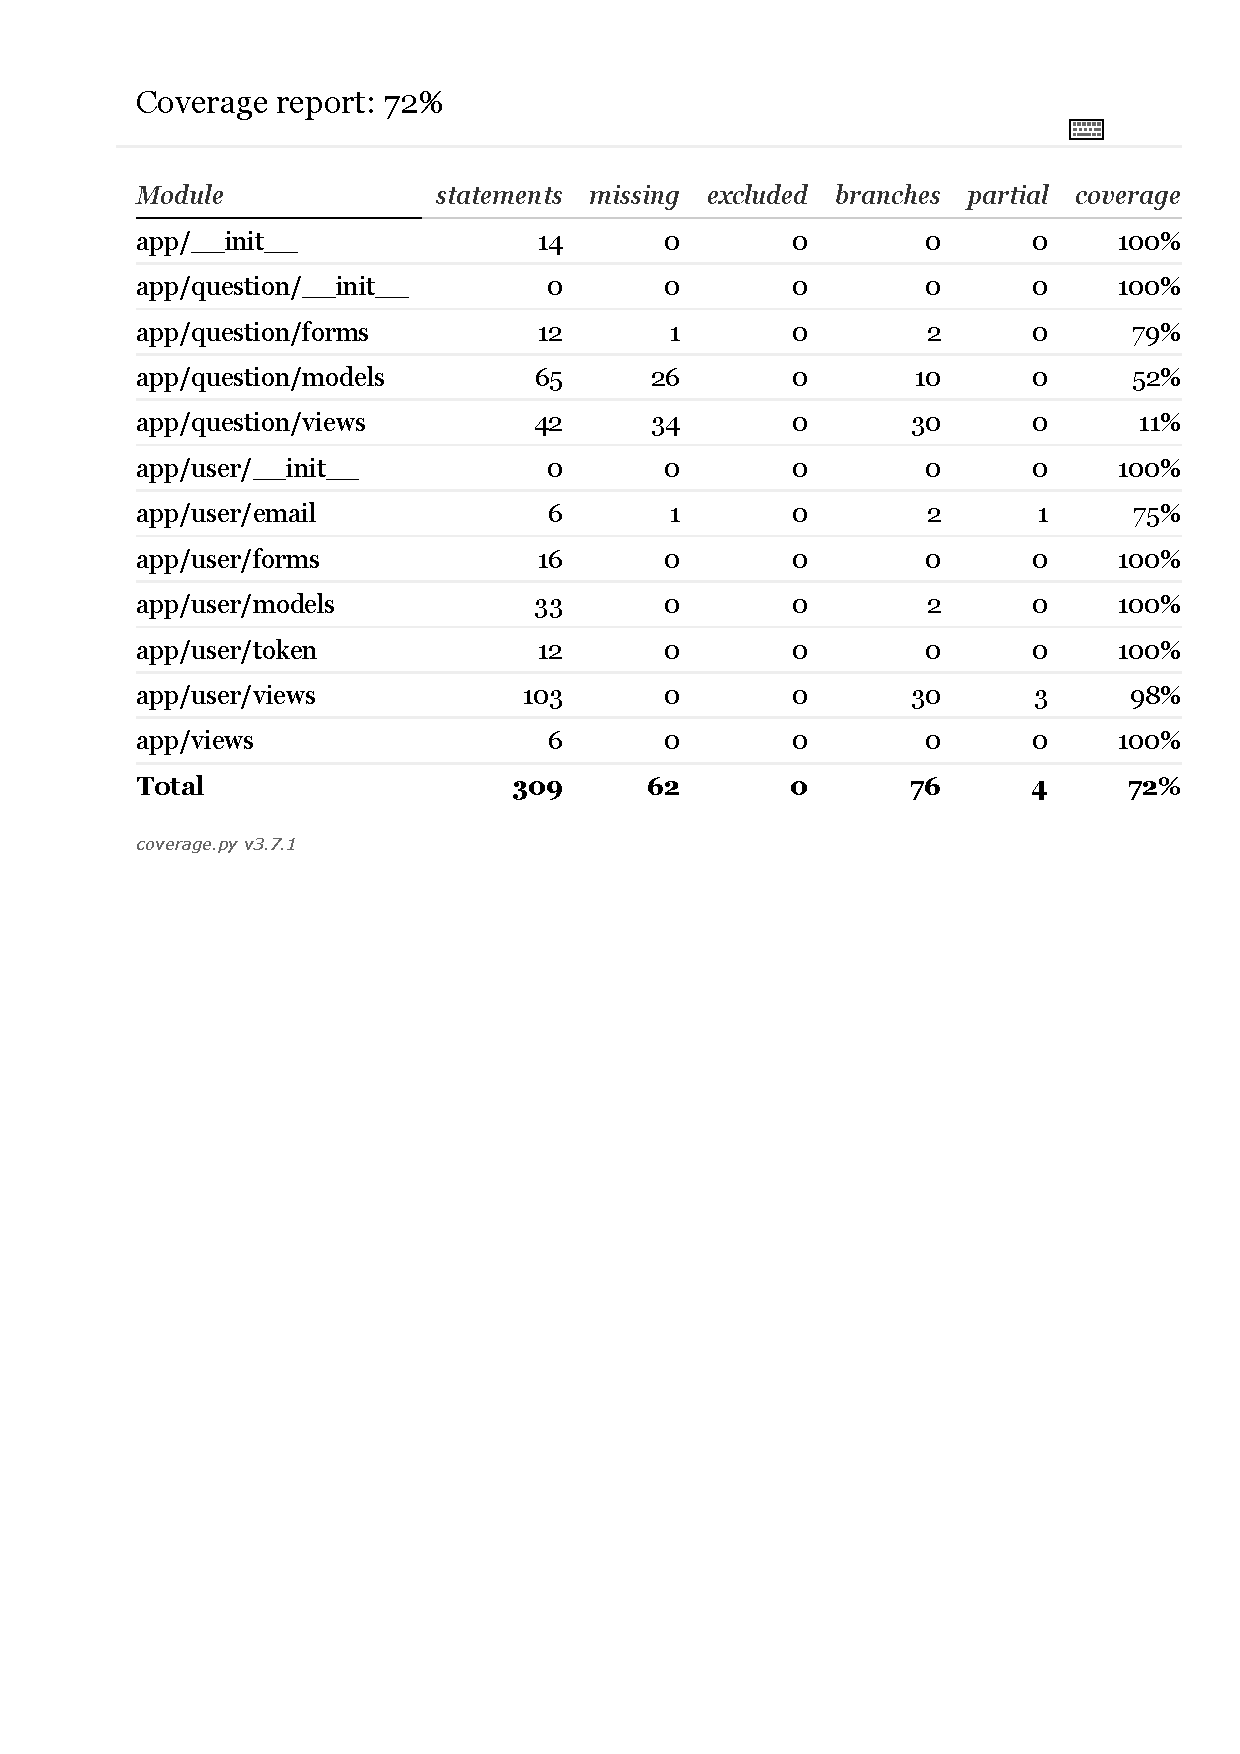
\includegraphics[width=1\linewidth]{figures/testcoverage.pdf}
    \caption{Oversigt over dækningsgraden af unittests. Det ses også hvor mange udtryk der er dækket af tests.}
    \label{fig:testcoverage}
\end{figure}

På Figur \ref{fig:code_coverage} ses hvordan værktøjet viser hvilke dele af koden der er dækket af tests, og hvilke der ikke er.

\begin{figure}[h]
    \centering
    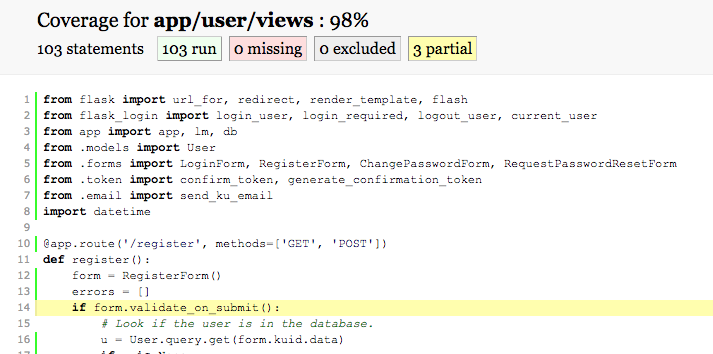
\includegraphics[width=1\linewidth]{figures/code_coverage.png}
    \caption{Eksempel på en grafik fremstilling, hvor et udtryk der kun delvist er dækket af tests fremhæves med gult.}
    \label{fig:code_coverage}
\end{figure}

\subsection{Integrationstests}
\label{sub:integrationstests}
Når vi har flere færdiggjorte moduler, så skal de testes sammen med realistiske input data, for at se om flere dele af systemet spiller sammen.

\subsection{Usability-tests}
\label{sub:usability_tests}
Når vi har en funktionsdygtig brugergrænseflade, så skal der udføres tests af hvor brugervenlig den er.
\FloatBarrier

\section{Brugergrænseflade og interaktionsdesign}
\label{sec:brugergraenseflade}
\subsection{Screenshots}
I Appendix \ref{sec:screenshots} ses screenshots af brugergrænsefladen for de vigtigste dele af vores projekt. De optræder i en rækkefølge der illustrerer dynamikken i en studerendes interaktion med vores system. I toppen af de fleste screenshots ses en navigationsbar, hvor man bl.a. kan se hvem der er logget ind, man kan logge ud og man kan ændre sit password. Der er desuden i venstre side et slags logo hvor man kan trykke for at blive taget tilbage til forsiden.

På Figur \ref{fig:screenshot_login} ses et screenshot af den første del af vores brugergrænseflade en studerende vil møde, nemlig en login skærm. Hvis man allerede er registreret som bruger kan man her indtaste sit KU-id og sit valgte kodeord, og dermed logge på systemet. Hvis man ikke er oprettet som bruger er der et link der tager en videre til registrering.

På Figur \ref{fig:screenshot_register} ses registreringssiden. Her kan man indtaste sit KU-id, vælge sig et kodeord og registrere sig. Systemet sender så en mail til den relevante KU-mail med et verificeringslink, og så snart den studerende har trykket på linket er vedkommende klar til at logge på systemet.

Når en studerende har logget sig ind i systemet vil vedkommende blive taget til index siden, som kan ses på Figur \ref{fig:screenshot_overview}. Her kan den studerende få et overblik over de forskellige \emph{thresholds} og de dertil hørende \emph{subjects}. Den studerende kan så vælge hvilket emne vedkommende vil arbejde på, og klikke på dets navn, hvilket fører dem videre til den næste del.

På Figur \ref{fig:screenshot_subject} ses \emph{subject} siden, hvor den studerende kan læse om det valgte emne, og hvis det virker interessant, trykke på knappen og begynde at løse opgaver inden for det bestemte emne. De dummy-data vi har i databasen på nuværende tidspunkt er lidt simple, så derfor ser siden også lidt kedelig ud lige nu.

Når den studerende har trykket \emph{begin} vil vedkommende blive stillet en række opgaver, f.eks. multiple choice opgaver som den der kan ses på Figur \ref{fig:screenshot_question}. Den studerende kan så afgive sit svar, enten ved at indtaste et svar, afkryde de korrekte bokse eller trække svarmulighederne hen på de korrekte positioner, og trykke på \emph{answer} knappen. Der er desuden mulighed for at den studerende kan få hints til opgaven, hvis det skulle være nødvendigt, ved at trykke på den dertilhørende knap.

Når den studerende har svaret på en opgave vil vedkommende blive taget til svar-siden, som kan ses på Figur \ref{fig:screenshot_answer}. Her får den studerende feedback på sit svar, der kan variere fra en helt simpel besked i form af rigtigt eller forkert til et mere detaljeret svar der f.eks. kunne indeholde en relevant stack trace. På svar-siden er der desuden et såkaldt \emph{Learn-O-Meter}, hvor den studerende kan se hvor langt vedkommende er nået med at gennemføre det valgte emne.

Endeligt vil den studerende når vedkommende har gennemført et emne blive taget til en sidste side, som kan ses på Figur \ref{fig:screenshot_finish}, hvor der som det ser ud lige nu ikke står meget andet end \emph{Done}. Den studerende kan så trykke på \emph{finish} knappen, hvilket vil tage vedkommende til index siden, og derfra kan vedkommende så vælge et nyt emne at arbejde på, eller vælge at logge ud.
\FloatBarrier

\subsection{AV-præsentation}
\label{sub:av_praesentation}

Der kan ses en præsentation af de vigtigste elementer i systemet på \url{https://youtu.be/JexAhDF9XCc}

\subsection{Tænke-højt forsøg}
\label{sub:taenke_hoejt}
Blah blah blah

\section{Projektsamarbejdet}
\label{sec:projektsamarbejdet}
Samarbejdet med kunden fungerer stadig ganske udemærket. Når vi mødes med dem er der en meget afslappet og munter stemning, og det virker som om vi er meget godt på bølgelængde sammen og forstår at diskutere og blive enige om de forskellige aspekter af projektet. Vi er stadig ikke så gode til at være officielle og tage referater og den slags, mest fordi møderne mere er en mundtlig samtale og diskussion af projektet, og de ting vi bliver enige om er sjældent helt nye for os, så det er tanker vi allerede selv har gjort os. Vi har desuden endnu ikke haft en helt fungerende prototype at vise frem og bruge som basis for en mere konkret diskussion af projektet, men det skulle vi gerne have klar til næste gang vi skal mødes med kunden.

Projektsamarbejdet internt i gruppen går nogenlunde, vi er ikke så gode til at holde sådan officielle møder  med dagsordener og referater og den slags, i stedet snakker vi bare sammen når vi lige mødes inde på universitetet, og arbejder på projektet når vi lige har tid, f.eks. i en pause eller en fri eftermiddag. Det meste af vores kommunikation foregår stadigvæk over email eller facebooks chat.

Vi har for nyligt oprettet en to-do liste inde i vores git repository, hvor vi prøver at notere de forskellige opgaver der mangler at blive løst, og som vi opdaterer løbende når vi får gennemført nogle af tingene eller støder på nye ting der skal laves. Det håber vi kan hjælpe os til at have et bedre overblik over projektet, og til at ikke glemme alle de små ting man måske støder på. På to-do listen er der tre sektioner, én til de store, vigtige ting, én til de mindre, mindre vigtige ting, og én til de ting der har at gøre med rapporten.

\newpage

\appendix
\section{Versionsstyring}
\label{sec:versionsstyring}
Link til github: \url{https://github.com/christiankjaer/pop-webhelp}

\subsection{Git log}
\label{sub:git_log}

\VerbatimInput[fontsize=\tiny]{git-log.txt}

\section{Changelog}
\label{sec:changelog}
\begin{tabular}{l l l}
08-04-2015 & CKL & Dokument oprettet. \\
14-04-2015 & CKL & Tilføjet use cases og krav. \\
16-04-2015 & LSE & Tilføjet UseCaseModel og BCE model. \\
16-04-2015 & CKL & Tilføjet review af Parnas og Clements. \\
17-04-2015 & TSH & Tilføjet review af Gould og Lewis. \\
17-04-2015 & LSE & Tilføjet Abstract og Projektsamarbejdet. \\
17-04-2015 & CKL & Tilføjet use cases, sekvensdiagram og klassediagram. \\
26-04-2015 & CKL & Tilføjet afsnit om tests. \\
30-04-2015 & CKL & Rettet til genaflevering og tilføjet systemdesign. \\
08-05-2015 & CKL & Tilføjet afsnit om strukturering. \\
10-05-2015 & LSE & Tilføjet Brugergrænseflade og screenshots, opdateret Systemdesign. \\
11-05-2015 & CKL & Tilføjet review af \cite{nsbullet}. \\
20-05-2015 & CKL & Tilføjet afsnit omkring systemdesign af brugere og begyndt på spørgsmål. \\
\end{tabular}

\section{Timeline}
\label{sec:timeline}
\begin{tabular}{l l p{8cm}}
11-03-2015 & Første møde med kunde: & Vi har første møde med kunden hvor vi snakker om hvad projektet går ud på og diskuterer krav og løsningsforslag. \\
16-04-2015 & Andet møde med kunde: & Vi har haft andet møde med kunden, hvor vi har snakket om modellen for de opgaver der skal være i systemet. \\
22-04-2015 & Internt møde i gruppen: & Vi har diskuteret databasemodeller, og vi er kommet frem til et databaseskema for denne iteration af systemet. Derudover fik vi udviklet i fællesskab på systemet. \\
27-04-2015 & Tredje møde med kunde: & Vi blev enige om en endelig funktionalitet for den første iteration af produktet. Derudover diskuterede vi udformingen af spørgmsålstyper og hvordan det hele skulle knyttes sammen. \\
07-05-2015 & Internt møde i gruppen: & Vi mødtes internt i gruppen for at diskutere udestående implementationsopgaver, og kigge på nogle ting sammen. \\
07-05-2015 & Første fungerende prototype: & Vores første fungerende prototype af vores projekt er færdig, hvor vi har fået bundet alle de elementer vi løbende har lavet sammen til et sammenhængende hele. Admin aspektet mangler stadig. \\
21-05-2015 & Endelige protype færdig: & Vi har færdiggjort vores endelige prototype med alle de store elementer på plads. \\
27-05-2015 & Afsluttende møde med kunde: & Vi havde vores endelige møde med kunden hvor vi præsenterede dem for vores seneste prototype. Kunden virkede imponeret, og vi diskuterede mulighederne for at arbejde videre på projektet. \\
\end{tabular}

\newpage

\bibliographystyle{alpha}
\bibliography{refs}{}

\newpage
\section{Brugergrænseflade screenshots}
\label{sec:screenshots}
\begin{figure}[h!]
    \centering
    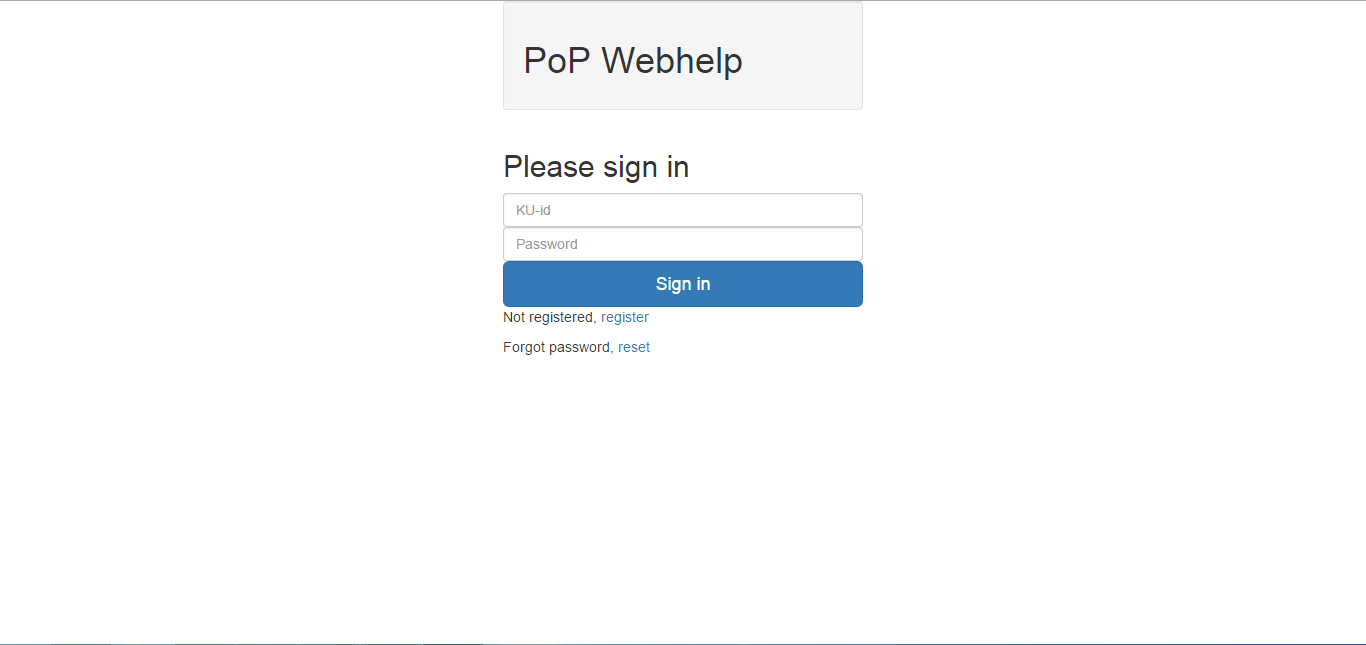
\includegraphics[width=1\linewidth]{figures/interface/login.png}
    \caption{Screenshot af login-siden.}
    \label{fig:screenshot_login}
\end{figure}


\begin{figure}[h!]
    \centering
    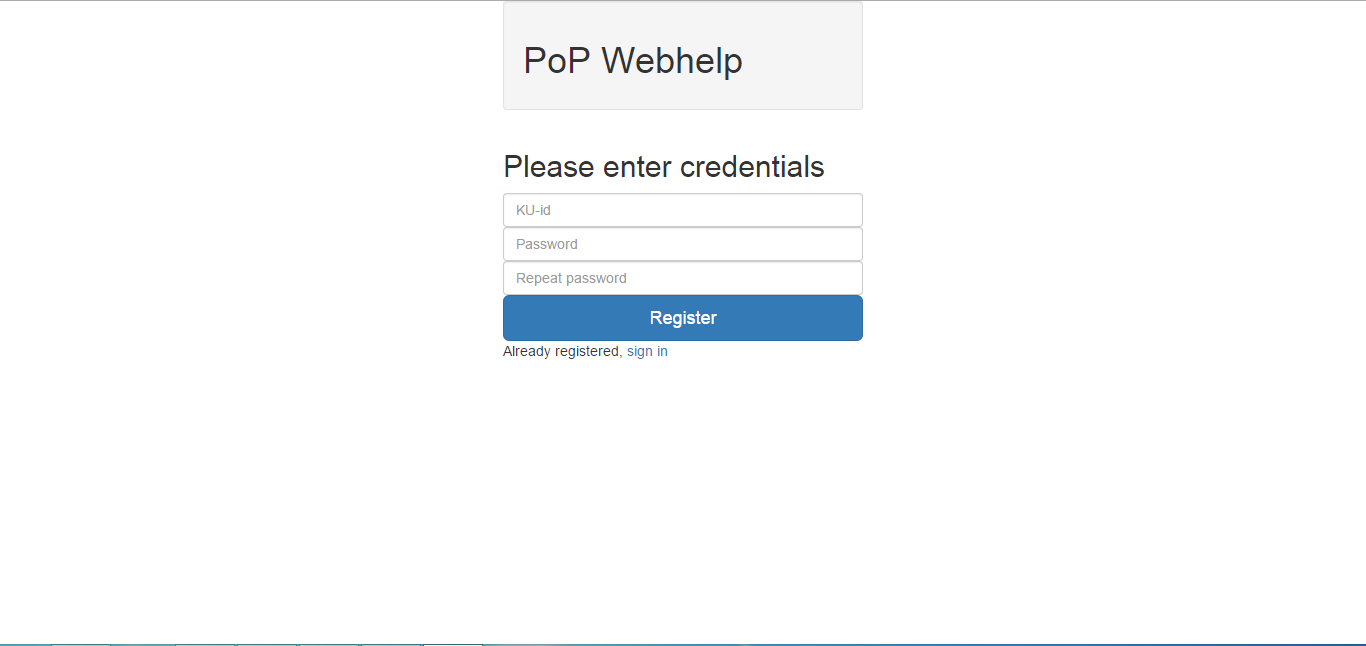
\includegraphics[width=1\linewidth]{figures/interface/register.png}
    \caption{Screenshot af registrerings-siden.}
    \label{fig:screenshot_register}
\end{figure}


\begin{figure}[h!]
    \centering
    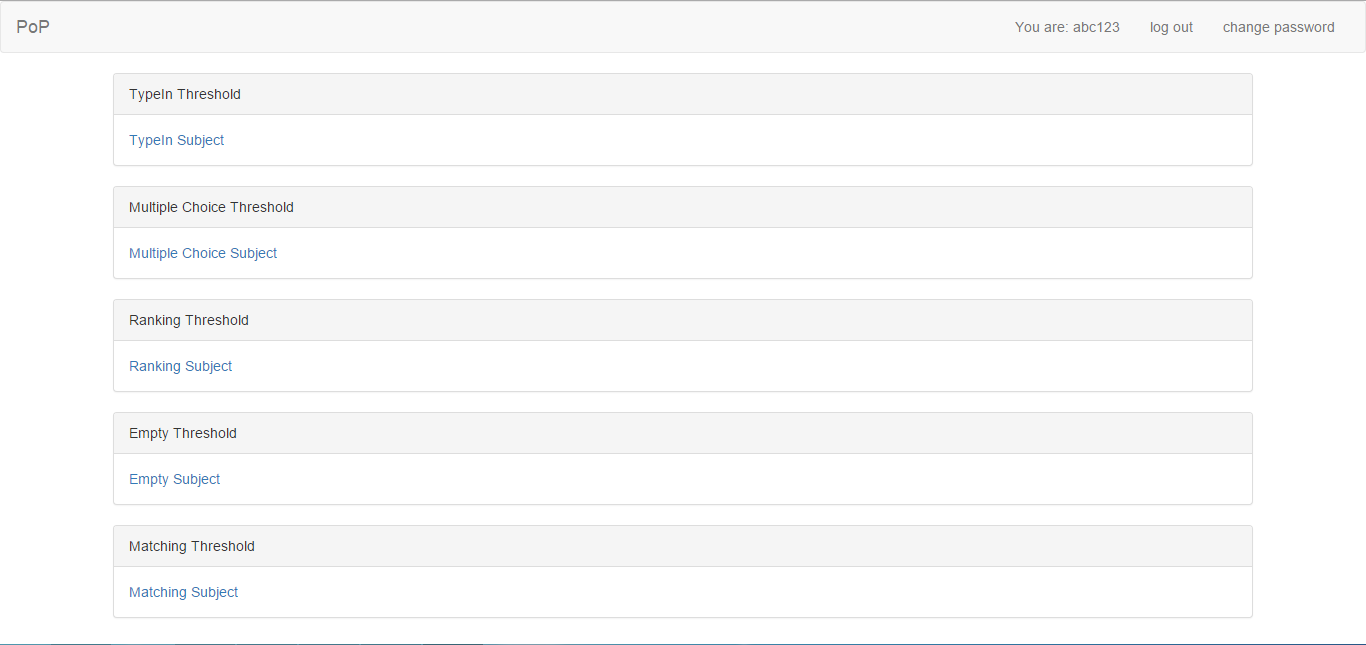
\includegraphics[width=1\linewidth]{figures/interface/overview.png}
    \caption{Screenshot af index-siden.}
    \label{fig:screenshot_overview}
\end{figure}


\begin{figure}[h!]
    \centering
    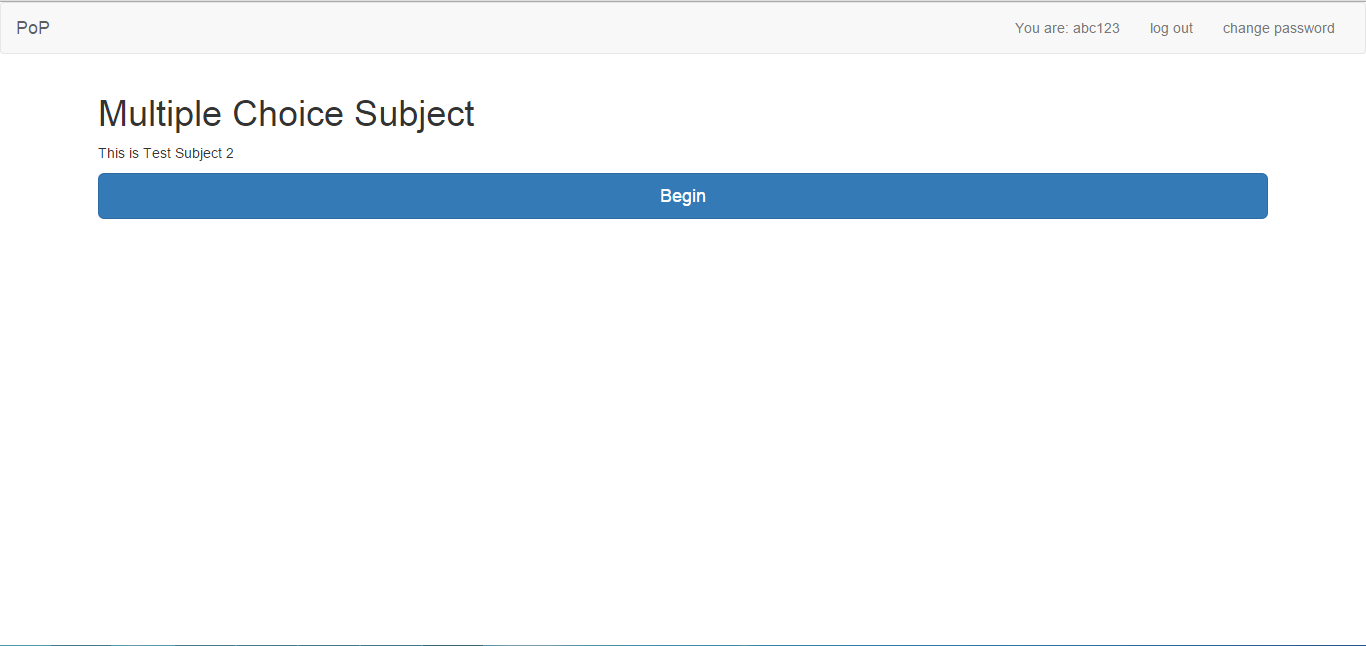
\includegraphics[width=1\linewidth]{figures/interface/subject.png}
    \caption{Screenshot af emne-siden.}
    \label{fig:screenshot_subject}
\end{figure}


\begin{figure}[h!]
    \centering
    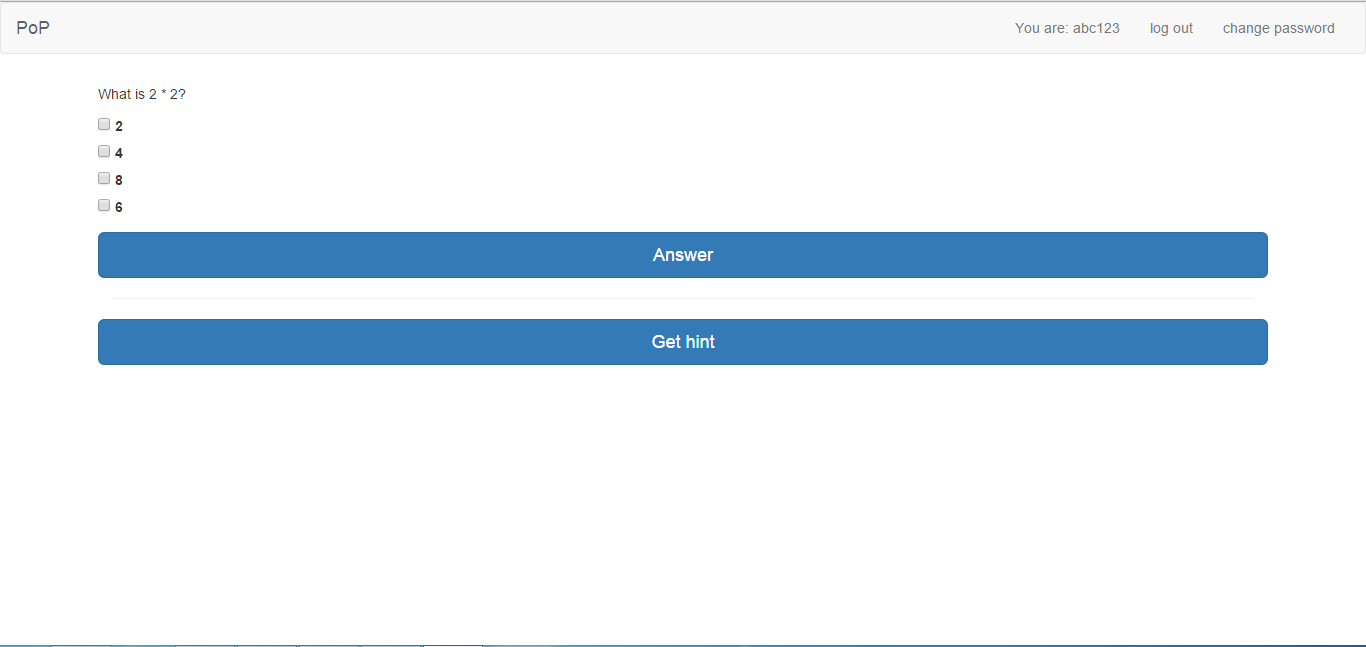
\includegraphics[width=1\linewidth]{figures/interface/question.png}
    \caption{Screenshot af spørgsmåls-siden.}
    \label{fig:screenshot_question}
\end{figure}


\begin{figure}[h!]
    \centering
    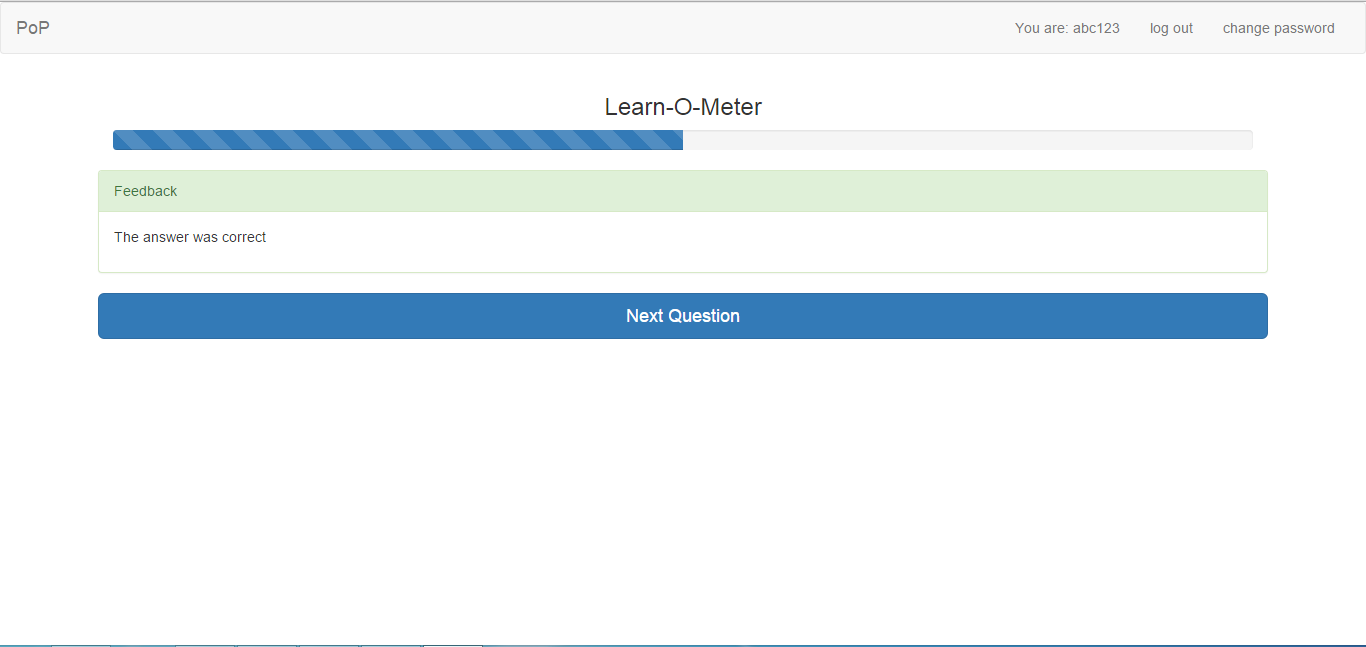
\includegraphics[width=1\linewidth]{figures/interface/answer.png}
    \caption{Screenshot af svar-siden.}
    \label{fig:screenshot_answer}
\end{figure}


\begin{figure}[h!]
    \centering
    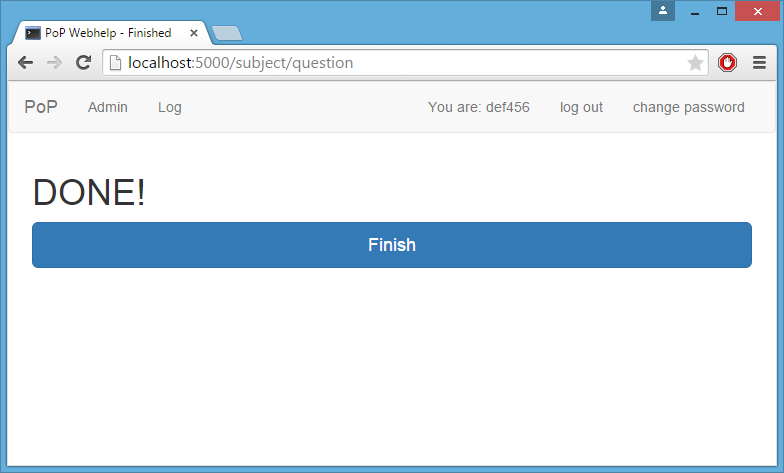
\includegraphics[width=1\linewidth]{figures/interface/finish.png}
    \caption{Screenshot af færdig-siden.}
    \label{fig:screenshot_finish}
\end{figure}

\end{document}
